\documentclass[11pt]{article}
\usepackage[margin=1in]{geometry}
\usepackage{volfit_preamble}
\usepackage{tikz}
\usetikzlibrary{arrows.meta,positioning,fit,backgrounds,calc}
\graphicspath{{figures/}}

\title{\textbf{System Overview, Conventions \& Hyperparameter Atlas}\\[2pt]
\large What the Vol-Fitter does, the pipeline, and the master index of every knob\\[2pt]
\normalsize Vol-Fitter Technical Notes, No.~00}
\author{Vol-Fitter}
\date{\today}

\begin{document}
\maketitle

\begin{abstract}
This is the map of the territory. The Vol-Fitter is an implied-volatility
surface fitter in the spirit of a professional vola-fitter, with one
differentiating capability: it \emph{extrapolates} sparse smile observations to
a full universe of smiles, across expiries \emph{and} assets, by propagating
signal through a graph whose nodes are smiles $(\text{underlying},T)$. This note
states the market and normalization conventions shared by the whole series,
walks the end-to-end compute pipeline (fetch $\to$ forwards/carry $\to$ prepare
[de-Americanize, screen, weight] $\to$ fit $\to$ views $+$ graph), catalogues
what the application can do, and ends with an index of the \emph{principal
calibration controls}, cross-linked to the topic notes that derive each knob.
It is the front door: read it once, then any other note in the series stands
alone.
\end{abstract}

\tableofcontents
\newpage

%======================================================================
\section{What the application is}
\label{sec:what}

At its core the Vol-Fitter solves one problem repeatedly --- \emph{given noisy,
sparse option quotes for one expiry of one underlying, produce a smooth
implied-volatility smile under explicit no-arbitrage control} --- and then
layers three ambitions on top of it:

\begin{enumerate}[leftmargin=1.6em]
\item \textbf{A choice of models, all arbitrage-aware.} Three slice
parametrizations share the per-expiry calibration spine --- the \emph{LQD}
log-quantile-density model (Note~01), \emph{SVI / SVI-JW} (Note~02), and the
\emph{Multi-Core Sigmoid (MCS)} family (Note~03) --- and a fourth model stands
apart: the \emph{piecewise-affine local-volatility surface} (Note~04), a
\emph{jointly} calibrated maturity~$\times$~strike grid whose unknown is
piecewise-affine local \emph{variance}, priced through the Dupire PDE. On
arbitrage the honest statement is graded: LQD is butterfly-free \emph{by
construction}; the LV surface is structurally arbitrage-clean (positive local
variance); SVI and MCS are \emph{soft-fenced} by sampled penalties and
explicitly diagnosed --- a penalty reduces but does not guarantee zero residual
violation, and the measured residual rates are reported per fit rather than
assumed away.
\item \textbf{A professional desk workflow.} Real bid/ask handling (fit to mid,
to the bid--ask band, or to a haircut band), var-swap targets, density-corrected
weighting, event time dilation, dividend and forward treatment, spot--vol
dynamics, a Bayesian prior-persistence machine that decides, feature by feature
(operator by operator), whether the live quotes identify a smile feature or the
saved prior should carry it, and a temporal observation filter (a per-handle
Kalman/MAP estimator, Note~15) that denoises noisy or contradictory quotes while
treating a genuine data gap as absent evidence rather than noise. The filter has
three modes: \texttt{off} (byte-identical to the feature never existing),
\texttt{overlay} (post-fit state and display update only), and \texttt{active}
(the prediction enters the calibration objective before optimization);
\texttt{active} is off by default and still carries a documented shock-day lag.
\item \textbf{Graph smile-extrapolation.} The headline differentiator (Note~14):
a transported prior plus the lit-node calibration innovation are propagated
through a \emph{directed Bayesian graph} --- optionally optimal-transport
regularized; the OT term is off by default ($\lambda=0$) --- to reconstruct the
\emph{dark} nodes.
\end{enumerate}

\begin{heuristic}
The unifying idea is that a volatility surface is not a curve to be drawn but a
\emph{family of probability laws} to be inferred --- one risk-neutral law per
$(\text{underlying},T)$ node --- subject to no-arbitrage couplings (butterfly
within a slice, calendar across expiries) and to a Bayesian prior that ties the
whole universe together. Every design choice in the app follows from taking that
sentence literally.
\end{heuristic}

\paragraph{Vocabulary.} Terms the whole series uses without ceremony, defined
once. A \emph{smile} is the implied-volatility curve of one
$(\text{underlying},T)$; a \emph{slice} is one smile's fitted model; a
\emph{surface} is all expiries of one underlying; a \emph{node} is one
$(\text{underlying},T)$ pair viewed as a graph vertex. A node is \emph{lit}
when its quotes are consumed and calibrated, and \emph{dark} otherwise ---
operationally, dark means the quotes are absent, unusable, deliberately
withheld, or simply not consumed; it does not necessarily mean nobody quoted.
The \emph{prior} is the saved previous fit, transported to today's market; the
\emph{innovation} is a lit node's fitted-minus-prior move. A \emph{handle} is a
scalar smile summary --- the three ATM handles are level $\sigma_0$, skew $s_0$
and curvature $\kappa_0$. The \emph{haircut band} is the bid--ask band shrunk
by a fixed vol amount; a \emph{vol bp} is $0.01$ vol point ($10^{-4}$ in
volatility); a \emph{WW smile} is a W-shaped smile (central trough with two
shoulders, Note~03). Abbreviations: CRR (Cox--Ross--Rubinstein binomial tree),
SSR (skew-stickiness ratio, Note~12), OT (optimal transport), MAP (maximum a
posteriori), GN (Gauss--Newton), NBBO (national best bid/offer).

\begin{invariant}
The system-wide contracts every note protects, stated once:
\begin{enumerate}[leftmargin=1.6em]
\item \textbf{Arbitrage-cleanliness is structural where possible, measured
where not.} LQD and the LV surface are clean by construction; SVI/MCS are
fenced by penalties that are exactly zero on admissible slices --- which bounds
but does not eliminate residual violation --- and the residual rates are
reported by explicit per-fit diagnostics, never assumed away.
\item \textbf{Every feature is strictly additive.} Bands, var-swap targets,
calendar coupling, the event clock, priors, betas, the wing penalty, the
observation filter: each is byte-identical to its absence when off --- and
that byte-identity is test-locked, not asserted.
\item \textbf{Numbers are measured, not copied.} Figures and tables are
generated fresh by the production code; reference listings are executed
against the modules they distill; claims carry test anchors.
\item \textbf{Versioned invalidation is scoped.} Editing one name's rate,
dividends, events or prior bumps that ticker's version only --- never the
universe. Whether the name then \emph{refits} immediately depends on the
workflow gate: with \texttt{autoCalibrate} on it refits in the background; on
the trigger-gated live server (which defaults \texttt{autoCalibrate} off) the
existing fit is kept, marked stale, and waits for an explicit Calibrate.
\end{enumerate}
\end{invariant}

\Cref{fig:guarantees} shows the two static-arbitrage checks, each in its
correct coordinates, on a four-expiry synthetic surface fitted by the
production LQD calibrator. Panel~(b) is the \emph{butterfly} check: every
implied density is non-negative, by construction. Panel~(c) is the
\emph{calendar} check: stacked \emph{total variance} $w(k,T)$, where for
forward-normalized (mean-one) slices absence of calendar arbitrage at fixed
log-moneyness is exactly the non-crossing ordering $w(k,T_{i+1})\ge w(k,T_i)$
at \emph{every} $k$ --- the same view the app's Stacked IV tab draws. Two
tempting substitutes are not checks at all: stacked \emph{vol} smiles carry
no calendar content ($\sigma$ mixes $w$ with the clock, so clean surfaces
cross freely in vol), and ATM-only monotonicity is necessary but far from
sufficient. The four slices here are fitted independently, so the displayed
dominance is \emph{measured} --- the generator asserts a positive minimum
inter-expiry gap on the displayed grid before writing the figure --- not
enforced; the enforcement coupling is Note~10's calendar machinery.

\begin{figure}[H]
\centering
\begin{minipage}{0.49\textwidth}\centering
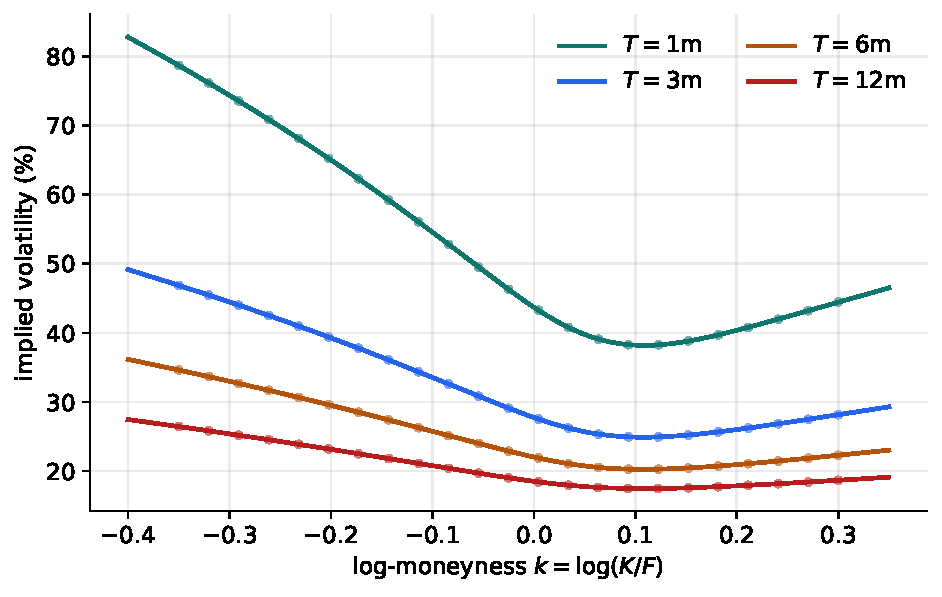
\includegraphics[width=\textwidth]{fig_ov_smiles.pdf}\\[2pt]
{\footnotesize (a) Four fitted smiles}
\end{minipage}\hfill
\begin{minipage}{0.49\textwidth}\centering
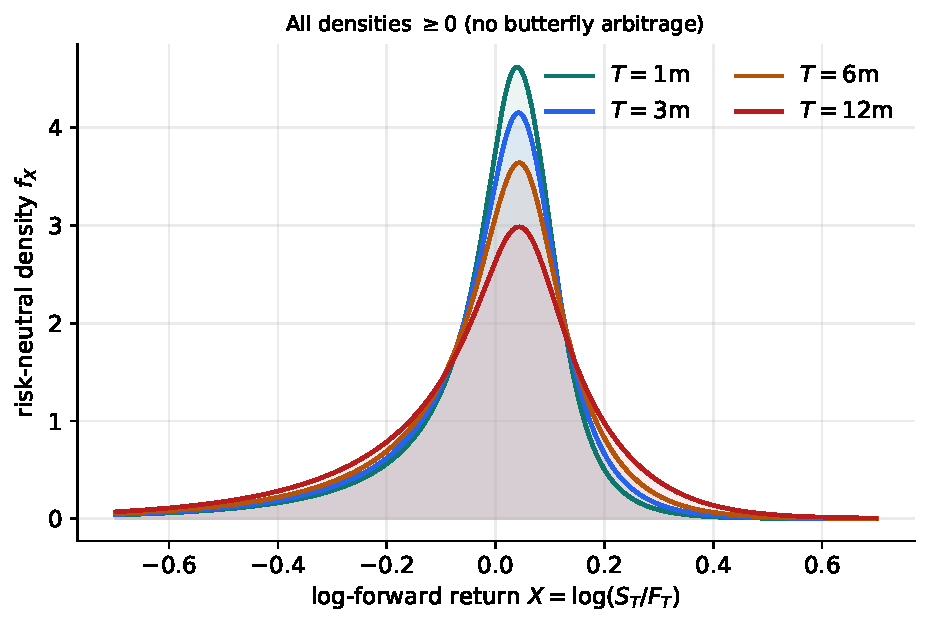
\includegraphics[width=\textwidth]{fig_ov_densities.pdf}\\[2pt]
{\footnotesize (b) Stacked densities, all $\geq 0$}
\end{minipage}
\\[6pt]
\begin{minipage}{0.62\textwidth}\centering
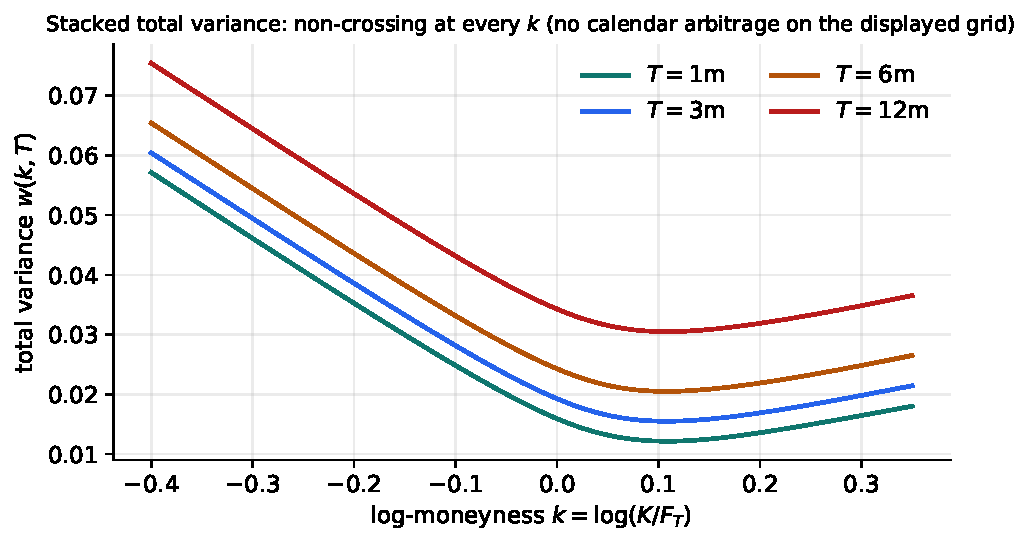
\includegraphics[width=\textwidth]{fig_ov_stackedvar.pdf}\\[2pt]
{\footnotesize (c) Stacked total variance: non-crossing at every $k$}
\end{minipage}
\caption{The two static-arbitrage checks, produced end to end by the
production LQD fitter on a synthetic calendar-monotone surface. Panels a, b:
the fits and their non-negative densities (no butterfly arbitrage, by
construction). Panel c: stacked total variance, non-crossing at every
displayed $k$ (no calendar arbitrage there --- measured on independently
fitted slices; enforcement is Note~10's coupling).}
\label{fig:guarantees}
\end{figure}

%======================================================================
\section{Market conventions and normalization}
\label{sec:conventions}

These conventions hold across the entire series; individual notes assume them
without restating.

\begin{definition}[Forward measure and normalization]
For expiry $T$ with forward price $F_T$, work under the $T$-forward measure and
in forward-normalized, undiscounted units. The log-moneyness is
$k=\log(K/F_T)$, the log-forward return is $X_T=\log(S_T/F_T)$, and normalized
call/put prices are $C_T(k)=\E^T[(e^{X_T}-e^k)^+]$ and
$P_T(k)=\E^T[(e^k-e^{X_T})^+]$, with the martingale condition $\E^T[e^{X_T}]=1$.
\end{definition}

\begin{definition}[Total variance and the Black map]
The normalized Black call is $\Black(k,w)=\PhiN(d_+)-e^k\PhiN(d_-)$ with
$d_\pm=-k/\sqrt w\pm\sqrt w/2$. Total implied variance $w(k,T)$ is the unique
$w$ solving $\Black(k,w)=C_T(k)$ --- a property of the \emph{price},
independent of any time convention; the fitter inverts it by a vectorized
scheme rather than a scalar root-find per strike. Annualizing $w$ by a clock
gives an implied volatility: $\sigma^2=w/t$ under the calendar clock,
$\sigma^2=w/\tau$ under the event clock below.
\end{definition}

This one primitive underlies every model in the series; in normalized form it is a
handful of lines (matches production to $10^{-12}$):

\begin{lstlisting}[caption={The normalized Black call $\Black(k,w)$ --- the shared
pricing primitive (distilled from \texttt{core/black.py}).},label={lst:black}]
def black_call(k, w):
    # k = log(K/F); w = total implied variance
    sq = np.sqrt(w)
    dp = -k/sq + 0.5*sq        # d_+;  d_- = d_+ - sqrt(w)
    price = norm_cdf(dp) - np.exp(k)*norm_cdf(dp - sq)
    intrinsic = np.maximum(1 - np.exp(k), 0.0)
    return np.where(w > 1e-12, price, intrinsic)
\end{lstlisting}

Three conventions deserve emphasis because they recur:
\begin{itemize}[leftmargin=1.4em]
\item \textbf{Two clocks, one $w$.} Four objects, kept distinct: $t$ is the
calendar year-fraction to expiry; $w$ is the clock-independent total variance
inverted from the price; $\sqrt{w/t}$ is the calendar-annualized \emph{market}
IV; $\sqrt{w/\tau}$ is the \emph{working} (event-time) IV, where $\tau$ is
calendar time dilated by scheduled events (Note~11). Fits live on $\tau$ when
the event clock is on. ``Adding an event lowers IV'' means precisely: at fixed
price (hence fixed $w$), the event raises $\tau$ and so lowers the
\emph{working} IV --- the market IV and the price are untouched.
De-Americanization and carry always run on the calendar clock $t$.
\item \textbf{Forward-normalized everything.} Prices, strikes and densities are
quoted relative to $F_T$, so a single smile object is spot-independent until a
dynamics rule (Note~12) transports it under a spot move.
\item \textbf{Residual units are per-model.} LQD and the LV surface calibrate
on price residuals divided by Black vega --- a volatility-like objective whose
every iterate is a valid price (Notes~01, 04, 07); SVI and MCS fit directly in
implied-volatility units. The bid--ask/haircut band objective (Note~07) is
expressed in vol space for all models.
\end{itemize}

%======================================================================
\section{The compute pipeline}
\label{sec:pipeline}

Every smile the app shows is the output of the pipeline in
\cref{fig:pipeline}. The stages are deliberately decoupled and independently
cached so that, e.g., editing a fit penalty never re-pulls data or re-runs
de-Americanization.

\begin{figure}[H]
\centering
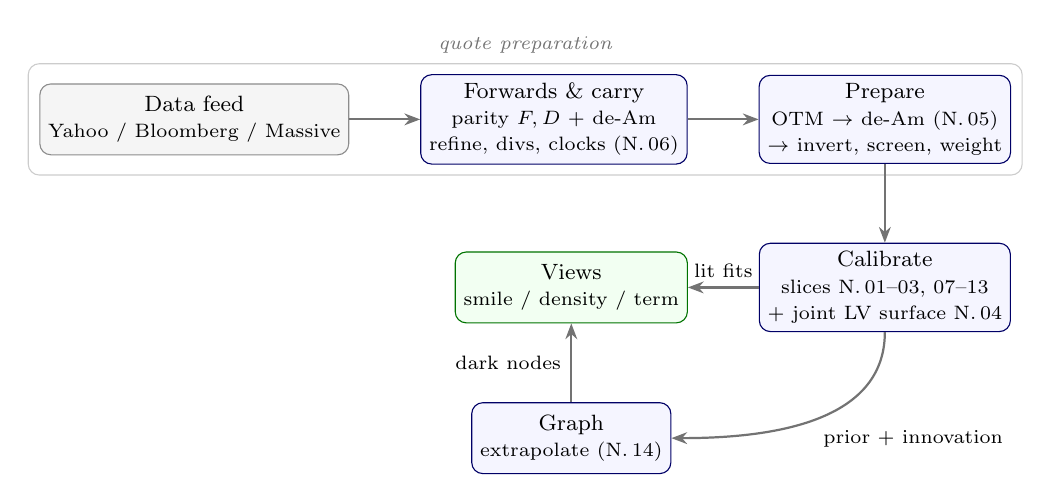
\begin{tikzpicture}[
  node distance=6mm and 9mm,
  box/.style={draw, rounded corners, align=center, minimum height=9mm,
    inner sep=3pt, font=\footnotesize, fill=blue!4, draw=blue!40!black},
  data/.style={box, fill=black!4, draw=black!45},
  view/.style={box, fill=green!5, draw=green!45!black},
  arr/.style={-{Stealth[length=2mm]}, thick, draw=black!55},
]
\node[data] (feed) {Data feed\\\scriptsize Yahoo / Bloomberg / Massive};
\node[box, right=of feed] (fwd) {Forwards \& carry\\\scriptsize parity $F,D$ + de-Am\\\scriptsize refine, divs, clocks (N.\,06)};
\node[box, right=of fwd] (prep) {Prepare\\\scriptsize OTM $\to$ de-Am (N.\,05)\\\scriptsize $\to$ invert, screen, weight};
\node[box, below=10mm of prep] (fit) {Calibrate\\\scriptsize slices N.\,01--03, 07--13\\\scriptsize + joint LV surface N.\,04};
\node[view, left=of fit] (views) {Views\\\scriptsize smile / density / term};
\node[box, below=10mm of views] (graph) {Graph\\\scriptsize extrapolate (N.\,14)};

\begin{scope}[on background layer]
  \node[draw=black!20, rounded corners, fit=(feed)(prep), inner sep=4pt,
    label={[font=\scriptsize\itshape, black!55]above:quote preparation}] {};
\end{scope}

\draw[arr] (feed) -- (fwd);
\draw[arr] (fwd) -- (prep);
\draw[arr] (prep) -- (fit);
\draw[arr] (fit) -- node[above,font=\scriptsize]{lit fits} (views);
\draw[arr] (fit.south) to[out=-90,in=0] node[below right,font=\scriptsize]{prior + innovation} (graph.east);
\draw[arr] (graph) -- node[left,font=\scriptsize]{dark nodes} (views);
\end{tikzpicture}
\caption{The end-to-end compute spine. The forward, discount, dividends and
clocks are resolved first (parity with an American de-bias refinement); quote
preparation then selects the OTM side, de-Americanizes each quote, and
inverts/screens/weights; calibration (per-expiry slices plus the jointly
fitted LV surface) feeds the lit views \emph{and} the graph extrapolator,
whose dark-node reconstructions feed the same views.}
\label{fig:pipeline}
\end{figure}

\paragraph{Stage by stage.}
\begin{enumerate}[leftmargin=1.6em]
\item \textbf{Data feed.} A provider registry exposes Yahoo (US options),
Bloomberg (xbbg; US + non-US indices/equities), and Massive (Polygon/OPRA), plus
a synthetic source; an as-of selector serves Live / previous-close / EOD /
captured-replay. US-options-only providers and the non-US Bloomberg path are
handled transparently.
\item \textbf{Forwards, dividends and clocks} (Note~06). Resolved \emph{before}
any per-quote work, because everything downstream consumes them. Put--call
parity on the raw chain yields the implied forward and discount (clamped
against feed noise); the forward inference itself contains a near-ATM American
de-bias loop, so the regressed forward is consistent with American quotes.
Discrete dividends and the two clocks --- calendar $t$ and event-dilated
variance time $\tau$ --- are resolved here too. One provider pathology is
handled upstream of the regression: chains a delayed feed \emph{synthesizes}
at zero carry (NBBO gated, so the provider emits Black prices from its own IV
marks at $F=$ spot, $D=1$) are flagged at capture and \emph{pinned} to
$F=$ spot, $D=1$ rather than parity-regressed --- regressing quotes that
already embed the provider's carry produced garbage forwards.
\item \textbf{Prepare} (Notes~05, 07). Per-expiry, given the resolved forward
and clocks: select the out-of-the-money side of each strike; then
\emph{de-Americanize} every kept quote (Note~05) --- listed equity options are
American, and each is converted to its European-equivalent implied volatility
by inverting a Cox--Ross--Rubinstein tree (bisection), with a Numba kernel for
wide chains and a content-digest cache so fit-tuning never re-runs it; then
normalize, invert to total variance (vectorized), apply the static
no-arbitrage/wing screen --- every dropped quote is quarantined with a reason,
never silently discarded --- run the wing-only, band-constrained convexity
repair (holding the ATM core fixed), and assign observation weights (Note~07).
\item \textbf{Calibrate.} The three parametric families fit per-expiry slices;
the LV surface is calibrated \emph{jointly} across maturities and strikes from
the same prepared quotes (Note~04). Each fit runs under the active objective:
mid / bid--ask band / haircut (Note~07), optional var-swap target (Note~08),
calendar coupling (Note~10), event clock (Note~11), and Bayesian prior
persistence (Note~13). The observation Kalman filter (Note~15) sequences by
mode: \texttt{off} adds nothing (byte-identical); \texttt{overlay} updates the
filtered state and display \emph{after} the fit commits; \texttt{active}
inserts the prediction prior into the calibration objective \emph{before}
optimization.
\item \textbf{Views.} Every smile-derived view --- smile, stacked densities,
stacked total variance, quantile density, term structure, local-vol surface,
SSR scenario --- follows the chosen model and is downsampled for the UI. Views
serve lit fits and, once the graph has run, the reconstructed dark nodes.
\item \textbf{Graph} (Note~14). The transported prior plus the lit-node
innovation propagate through the directed Bayesian graph (OT term optional,
off by default) to reconstruct dark-node smiles with credible bands, which
flow back into the views.
\end{enumerate}

%======================================================================
\section{The smile graph}
\label{sec:graph}

The object that makes the app more than a slice fitter is the \emph{smile graph}
(\cref{fig:smilegraph}): nodes are smiles $(\text{underlying},T)$; edges encode
that one node informs another. Calendar edges link expiries of one name;
cross-asset edges link an index or sector ETF to its single names. A user marks
nodes \emph{lit} (quoted, calibrated) or \emph{dark} (to be reconstructed). The
graph carries the three ATM handles $(\sigma_0,s_0,\kappa_0)$ of each node as a
Gaussian signal and propagates the lit innovation to the dark nodes. Three
scalars do not make a smile: a dark node's full curve is obtained by
\emph{retargeting} --- the node's transported prior smile (a complete curve,
wings and all) is re-expressed in an ATM-orthogonal chart and its three handles
are moved to the posterior values, leaving the prior's shape modes (wings,
event convexity) untouched, so every reconstructed slice remains a valid
arbitrage-clean smile. Note~14 develops the directed Bayesian solver behind
the propagation (with an optional optimal-transport regularization, off by
default: \texttt{graphLambdaScale}$\,=0$) and the leave-one-out backtest that
measures its skill.

Two scoring conventions, used everywhere the graph is evaluated: \emph{skill}
is the reduction in held-out ATM error versus the transported-prior baseline,
in ATM vol bps --- positive means the graph beat mechanical transport; $\zeta$
is the standardized held-out residual (realized error divided by the posterior
credible band), so $\operatorname{std}\zeta=1$ means the bands are honest,
$>1$ overconfident (too narrow), $<1$ conservative. Skill is measured at
scale: on the 25-asset benchmark across three historical regimes ($\sim$47k
held-out scores), neighbour-supported indexes gain $+10$ to $+76$ ATM vol bps
over the transported-prior baseline and ETFs $+3$ to $+7$; fully-dark single
names behind lit indexes/ETFs --- the product case --- gain $+7.9$ to $+14.2$
bps in the August-2024 spike and $+3.8$ to $+7.2$ fully out-of-sample in the
October-2022 bear, with unbiased standardized residuals. In the calm July-2023
regime the dark-name skill is $\approx0$ (never negative): single-name moves
there are earnings-idiosyncratic, and the graph carries shared repricing, not
idiosyncratic news. The one weakness that measurement flagged --- calm-regime
dark-name bands at $\operatorname{std}\zeta\approx1.9$, overconfident --- is
now closed for the ATM level: an \emph{idiosyncratic band floor} (a strictly
causal floor built from the node's own trailing unexplained moves while lit,
on by default in production) moved the two calm cells $1.91\to1.02$ and
$1.85\to1.03$ with the posterior mean untouched. Widening the skew/curvature
bands in idiosyncratic tape remains open (Note~14).

\begin{figure}[H]
\centering
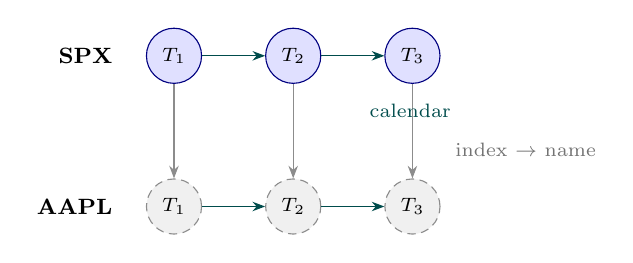
\begin{tikzpicture}[
  lit/.style={circle, draw=blue!50!black, fill=blue!12, minimum size=7mm,
    font=\scriptsize},
  dark/.style={circle, draw=black!45, fill=black!6, minimum size=7mm,
    font=\scriptsize, densely dashed},
  e/.style={-{Stealth[length=1.6mm]}, draw=black!45},
  cal/.style={e, draw=teal!60!black},
]
% index row (lit)
\node[lit] (i1) {$T_1$};
\node[lit, right=8mm of i1] (i2) {$T_2$};
\node[lit, right=8mm of i2] (i3) {$T_3$};
\node[left=3mm of i1, font=\footnotesize\bfseries] {SPX};
% name row (dark)
\node[dark, below=12mm of i1] (n1) {$T_1$};
\node[dark, right=8mm of n1] (n2) {$T_2$};
\node[dark, right=8mm of n2] (n3) {$T_3$};
\node[left=3mm of n1, font=\footnotesize\bfseries] {AAPL};
% calendar edges
\draw[cal] (i1) -- (i2); \draw[cal] (i2) -- (i3);
\draw[cal] (n1) -- (n2); \draw[cal] (n2) -- (n3);
% cross-asset edges (index informs name)
\draw[e] (i1) -- (n1); \draw[e] (i2) -- (n2); \draw[e] (i3) -- (n3);
\node[font=\scriptsize, teal!60!black] at (3.0,-0.7) {calendar};
\node[font=\scriptsize, black!55, anchor=west] at (3.45,-1.2) {index $\to$ name};
\end{tikzpicture}
\caption{A fragment of the smile graph: lit index nodes (solid) inform dark
single-name nodes (dashed) across both calendar and cross-asset edges. The graph
posterior reconstructs the dark smiles from the lit innovation.}
\label{fig:smilegraph}
\end{figure}

%======================================================================
\section{Capability catalogue}
\label{sec:capabilities}

\Cref{tab:caps} indexes what the app can do against the note that documents the
mathematics. It doubles as a reading order.

\begin{longtable}{p{0.36\textwidth}p{0.50\textwidth}r}
\caption{Capability $\to$ note index.}\label{tab:caps}\\
\toprule
Capability & Summary & Note\\
\midrule
\endfirsthead
\toprule Capability & Summary & Note\\ \midrule
\endhead
LQD smile model & Arbitrage-free-by-construction log-quantile density;
analytic Jacobian & 01\\
SVI / SVI-JW & Raw and jump-wing SVI with no-arb penalty and Lee cap & 02\\
Multi-Core Sigmoid (MCS) & Sigmoid base + zero-wing hats for WW/event smiles & 03\\
Local volatility & Jointly calibrated piecewise-affine local-\emph{variance}
surface (Dupire); GN/Numba calibration & 04\\
De-Americanization & CRR tree + bisection, Numba kernel, cache digest, wing convex repair & 05\\
Forwards / dividends & Parity forward + discount clamp, discrete divs & 06\\
Weighting \& bid--ask & Equal / time-value-density weights; band/haircut fit & 07\\
Variance-swap targets & Replication, LQD closed form, source-PDE & 08\\
Wings \& Lee bounds & Tail control unified across models & 09\\
Calendar arbitrage & Convex-order soft hinge, model-agnostic & 10\\
Event variance clock & Dual calendar/variance time, day-weighted events & 11\\
Spot--vol dynamics & Sticky strike/moneyness/local-vol, SSR transport & 12\\
Prior persistence & 7-mode Bayesian menu, precision gate, two-pass & 13\\
Graph extrapolation & Transported prior + directed increments + backtest & 14\\
Observation Kalman filter & Per-handle temporal denoising of the ATM handles;
one-stage MAP active mode & 15\\
\bottomrule
\end{longtable}

\paragraph{Viewer and data capabilities (engineering, not derived here).} The
workspace is organized into eight tabs --- Parametric, Local Vol, Forwards,
Options, Graph, Quality, Universe and View: charts of prior/current fit vs.\
quote bands in normalized or fixed strike, quantile and density functions, term
structure and event-dilated calendar in vol and variance, var-swap levels,
interactive quote select/erase/amend, universe selection, lit/dark node maps,
and the graph editor. The Quality tab aggregates publish-readiness per node
(fit quality, arbitrage diagnostics, data-age staleness) and drives the
export/reporting path. Data plumbing (providers --- including Massive intraday
history via flat files where entitled --- as-of replay, dividend editor,
persistence of named universes and fit history) is described in the project
README rather than in this mathematical series.

\begin{remark}[Current scope and limits]
What the application is \emph{not}, as of this writing. The live universe is
desk-scale: validation ran on a 25-asset, three-regime benchmark, and the graph
solver is dense --- comfortable to a few thousand nodes; a sparse solver is
deferred until a universe needs it. The server is a single-process application
state, deployed hosted single-tenant first; market-data entitlements are
bring-your-own. Sub-daily expiries (0DTE) are research-grade, not certified.
The app fits, extrapolates and publishes vanilla implied-vol surfaces: it does
not price or risk-manage exotics, route orders, or forecast --- dividends,
borrow and forwards are inputs or option-implied estimates, never predictions.
\end{remark}

%======================================================================
\section{The design rules that recur}
\label{sec:rules}

Reading the series end to end, a handful of design rules appear again and
again --- each learned from a production incident, each now documented as a
\emph{case file} in its note. They are worth stating once as the app's
engineering philosophy.

\begin{enumerate}[leftmargin=1.6em]
\item \textbf{The confinement principle} (Note~09). A constraint comparing
\emph{two} curves is sampled only where data pins both; a constraint
intrinsic to \emph{one} curve holds everywhere, wings included. Four
instances: the calendar floor (confined, Note~10), the LV convex wing
(confined, Note~04), the MCS Durrleman penalty (extended, Note~03), the
de-Am convexity repair (extended, but its \emph{authority} confined to the
quoted band, Note~05).
\item \textbf{Trust the well-identified parameter.} The parity forward keeps
the price level and refuses the noisy slope (Note~06); the prior gate trusts
the market exactly where quotes identify a feature and yesterday exactly
where they do not (Note~13).
\item \textbf{Persist shape, not level.} Operators and factors are
level-invariant baskets, so an overnight jump is never damped
(Note~13); the graph propagates \emph{increments}, so ``no change'' is the
default dark-node answer (Note~14).
\item \textbf{Route each model through its native object.} The var-swap is
a closed form for LQD, arithmetic for SVI/MCS, a source PDE for LV
(Note~08); the calendar constraint is the asset share for LQD and a
total-variance hinge for the overlays (Note~10). Uniform implementations
across non-uniform models are a trap.
\item \textbf{Measure first, fix second.} The short-dated LV failure was
convicted by per-expiry counts before any model change (Note~04); the MCS
wing penalty sits where the arb census located the violations (Notes~03,
09); the temporal backtests score priors, the graph and the observation
filter against honest held-out baselines (Notes~13--15).
\end{enumerate}

\Cref{tab:casefiles} indexes the production incidents documented across the
series --- the fastest way to learn the system is arguably to read these
first.

\begin{longtable}{p{0.52\textwidth}p{0.30\textwidth}r}
\caption{Case-file index: production incidents and their lessons.}\label{tab:casefiles}\\
\toprule Incident & Lesson & Note\\ \midrule
\endfirsthead \toprule Incident & Lesson & Note\\ \midrule \endhead
The six-day weekly that broke the LV strike grid (fit RMS
$108\to23.5$ vol bp after the fix) &
measure first; per-expiry coverage floors & 04\\
The convex wing that flattened SPY (fit RMS $25.7\to2.6$ vol bp once the
constraint left the quoted range) &
constraints stay off quoted territory & 04\\
The reverted global de-Am repair (ATM smile gap) &
repairs need confined authority & 05\\
The delayed feed that gapped the ATM smile (discount clamp; failed
rate-anchor) & trust the well-identified parameter & 06\\
The fit that took minutes (var-swap replication in the Jacobian) &
native-object routing & 08\\
The MCS that invented a put wing (R3$\times$R6 ablation, in-sample RMS:
input repair alone $92\to25$ vol bp, output penalty alone $749$, both
together $225$ with the violation gone) & input repair and output penalty
compose & 09, 03\\
The phantom calendar (NVDA/SPY flattened; the $151$-vol-bp flattening
reproduced, then $\to0$ under confinement) &
the confinement principle & 10, 09\\
The jump the strike anchor damped (operators persist shape) &
persist shape, not level & 13\\
The backtest that confirmed the hybrid default ($\sim$32 vol bp better on
the held-out wing, 1117 nodes) & defaults are chosen by held-out
evidence & 13\\
The transient-name topology defect (cross-asset skill exactly $0.000$ bp) &
exact zeros are disconnection, not damping & 14\\
The close-strike contradiction vs.\ the true gap (per-handle Kalman gains
level/skew/curvature $=0.80/0.72/0.03$: high where quotes contradict, near
zero where they are simply absent) & noise is not a gap: filter and prior
split the work & 15\\
The off-diagonal blow-up on coarse chains (cross-handle updates moved ATM
vol by $3$--$28$ vol \emph{points}) &
per-handle updates; caps do not police cross-gains & 15\\
\bottomrule
\end{longtable}

%======================================================================
\section{How the notes are organized}
\label{sec:org}

The topic notes, 01--15, are standalone and follow a common skeleton,
codified in the series style guide
(\texttt{Docs/notes/STYLE\_GUIDE.md}): an opening that states the
\emph{production problem} and the \emph{invariants} being protected (the
amber box near the top of every note), a theorem-shaped body whose central
object gets the note's single boxed equation, a worked example or
\emph{case file} told as a production incident, a \emph{traceability table}
tying each claim to its module and locking test, and three appendices ---
\textbf{A, a hyperparameter atlas} (every knob, surfaced or hidden, with its
default), \textbf{B, performance} (measured optimizations, including the
rejected ones), and \textbf{C, a reference implementation} ($\le50$ lines,
executed against the production module before being committed). Figures run
through the shared \texttt{figures/style.py} and their captions state the
lesson, not the axes. Notes cross-reference each other (this note's
\cref{tab:caps} is the index) but never depend on one another's internals.
Numbers and plots are \emph{measured}, not copied: where a fresh run differs
from an older design note, the fresh run wins. This overview is the deliberate
exception to the skeleton --- it is a map, not a theorem, so it carries no
boxed central equation, no traceability table and no performance or
reference-implementation appendix; its single appendix is the control index
below.

%======================================================================
\appendix
\section{Principal calibration controls}
\label{app:master}

A \emph{curated} index of the principal tunable parameters: surfaced (the
user-facing \texttt{FitSettings} and \texttt{OptionsSettings}) and hidden
(internal constants). It is deliberately not exhaustive --- the single source
of truth is the Pydantic schema pair in \texttt{volfit/api/schemas.py}, whose
field docstrings state each knob's unit, activation condition and effect, plus
each topic note's Appendix~A. (Workflow and data-fetch controls ---
spot polling, chain refetch cadence, streaming refit --- live in the same
schema and are omitted here as non-calibration knobs.) Each row points to the
note that derives its role; defaults are the shipped values. This is a
directory, not a derivation --- consult the referenced note for meaning.

\small
\setlength{\tabcolsep}{4pt}
\begin{longtable}{p{0.34\textwidth}p{0.14\textwidth}p{0.38\textwidth}r}
\caption{Surfaced parameters (principal; the schema is exhaustive).}\label{tab:master_surfaced}\\
\toprule
Parameter & Default & Role & Note\\
\midrule
\endfirsthead
\toprule Parameter & Default & Role & Note\\ \midrule
\endhead
\texttt{model} & \texttt{lqd} & smile family: \texttt{lqd} / \texttt{svi} /
\texttt{sigmoid} (MCS) & 01--03\\
\texttt{nOrder} & $6$ & LQD Legendre order & 01\\
\texttt{regLambda} / \texttt{regPower} & $10^{-6}$ / $1$ & LQD high-order ridge & 01\\
\texttt{barrierCenter} / \texttt{barrierScale} & $0.90$ / $50$ & LQD $A_R$ barrier & 01\\
\texttt{nCores} & $2$ & MCS hat count (schema-clamped at 2) & 03\\
\texttt{sigmoidRidge} & $10^{-2}$ & MCS hat-amplitude ridge & 03\\
\texttt{sivWingPenaltyPct} & $100$ & MCS put-wing Durrleman penalty ($0=$ off) & 03\\
\texttt{sviPenaltyWeight} & $10^{3}$ & SVI no-arbitrage penalty & 02\\
\texttt{leeSlopeMax} & $2.0$ & SVI Lee wing-slope cap & 02, 09\\
\texttt{fitMode} & \texttt{mid} & mid / bidask / haircut & 07\\
\texttt{weightScheme} & \texttt{equal} & equal / tv-density weights & 07\\
\texttt{haircut} & $0.005$ & band haircut (vol) & 07\\
\texttt{midAnchorWeight} & $0.05$ & band mid anchor & 07\\
\texttt{varSwapEnabled} & on & var-swap quotes surfaced + penalized & 08\\
\texttt{varSwapWeightPct} & $10\%$ & var-swap budget & 08\\
\texttt{varSwapMethod} & \texttt{static} & LV model var-swap: strike replication /
source PDE & 08\\
\texttt{enforceCalendar} & on & ascending-$T$ calendar coupling of Calibrate & 10\\
\texttt{calendarWeight} & $10^{6}$ & calendar soft-constraint penalty & 10\\
\texttt{extrapEnforce} & off & tapered no-arb enforcement in the extrapolated
region (advisory measurement always on) & 09, 10\\
\texttt{eventsEnabled} & on & event variance-clock master switch & 11\\
\texttt{normalizeEvents} & off & rescale so the 1Y day-weight budget stays 365 & 11\\
\texttt{gridStrikeMode} & \texttt{delta} & LV strike-vertex placement
(\texttt{delta} / \texttt{linear}) & 04\\
\texttt{gridXNodes} & $12$ & LV strike vertices --- a \emph{floor} in delta
mode, exact only in linear mode & 04\\
\texttt{gridXMinPerExpiry} & $8$ & LV short-dated coverage floor & 04\\
\texttt{gridTNodes} & $10$ & \emph{floor} on positive LV time vertices (the
base set --- $0$, pre-front node, every lit expiry --- is always kept) & 04\\
\texttt{gridRegLambda} / \texttt{gridRegRho} & $10^{-2}$ / $1$ & LV roughness penalty / ratio & 04\\
\texttt{convexWingWeight} & $10^{3}$ & LV wing-convexity penalty
(\texttt{convexWing} off by default; tail-confined) & 04\\
\texttt{frontTieWeight} & $10^{-2}$ & ties the free $t=0$ row to the first
data-identified row & 04\\
\texttt{lvVolCapMult} & $3.0$ & LV local-vol cap multiple & 04\\
\texttt{leftWingSlopeMult} & $1.5$ & LV left-wing extrapolation slope multiple & 04\\
\texttt{timeScheme} & \texttt{implicit} & LV PDE time scheme
(\texttt{rannacher} opt-in) & 04\\
\texttt{lvSolver} & \texttt{gn} & LV solver: matrix-free GN / scipy trf & 04\\
\texttt{lvFastKernel} & on & Numba vectorized-Thomas Dupire march & 04\\
\texttt{lvEarlyStop} & on & LV cold-fit early stop at the RMS stall & 04\\
\texttt{localVolEnabled} & on & LV calibration + workspace master switch & 04\\
\texttt{dynamicsRegime} & \texttt{sticky\_strike} & spot--vol regime seed & 12\\
\texttt{ssr} & $2.0$ & SSR value of the \texttt{custom} regime (inert
otherwise) & 12\\
\texttt{priorPersistenceMode} & \texttt{hybrid} & prior mode selector & 13\\
\texttt{priorOperatorSet} & ATM, RR25, BF25, VarSwap & operators to persist & 13\\
\texttt{priorOperatorStrengthPct} & $50\%$ & operator prior budget & 13\\
\texttt{priorOperatorRequiredPrecision} & $1.0$ & operator activation gate & 13\\
\texttt{priorOperatorGapExponent} & $1.0$ & gate exponent $\gamma$ & 13\\
\texttt{priorOperatorBandwidth} & $0.06$ & operator leg KDE bandwidth & 13\\
\texttt{priorOperatorCovarianceMode} & \texttt{diagonal} & operator covariance
route (\texttt{full} = Jacobian-propagated) & 13\\
\texttt{priorDataOnlyPrepass} & off & two-pass activation (measure precision
data-only, then refit) & 13\\
\texttt{priorFactorSet} & ATM, skew, curvature, VarSwap & smile factors to persist & 13\\
\texttt{priorFactorStrengthPct} & $50\%$ & factor prior budget & 13\\
\texttt{priorTailAnchorStrengthPct} & $20\%$ & hybrid tail-anchor budget & 13\\
\texttt{priorAnchorWeightPct} & $50\%$ & strike-gap prior budget & 13\\
\texttt{graphKappaScale} $\kappa$ & $1.0$ & graph temporal precision & 14\\
\texttt{graphEtaScale} $\eta$ & $1.0$ & graph directed smoothness & 14\\
\texttt{graphLambdaScale} $\lambda$ & $0.0$ & graph OT regularization ($0=$ OT
term off) & 14\\
\texttt{graphNu} $\nu$ & $0.1$ & graph UOT source allowance & 14\\
\texttt{idioFloor} & on & dark-node idiosyncratic credible-band floor & 14\\
\texttt{observationFilterMode} & \texttt{off} & filter off / overlay / active (MAP) & 15\\
\texttt{filterCovarianceMode} & \texttt{jacobian} & measurement-covariance route & 15\\
\texttt{filterProcessVolBpSqrtDay} & $30$ & ATM clock process noise (bp/$\sqrt{\text{day}}$) & 15\\
\texttt{filterProcessSkewSqrtDay} & $0.02$ & skew clock process noise & 15\\
\texttt{filterProcessCurvSqrtDay} & $0.05$ & curvature clock process noise & 15\\
\texttt{filterTransportNoiseScale} & $0.10$ & process std per unit transport distance & 15\\
\texttt{filterResidualInflation} & on & contradiction reads as measurement noise & 15\\
\texttt{filterAdaptiveSigma} & $3$ & innovation-gated adaptive $Q$ ($0=$ off) & 15\\
\texttt{filterMaxGain} & $1.0$ & per-handle own-gain safety cap & 15\\
\texttt{filterResetHours} & $96$ & maximum data gap predicted across & 15\\
\texttt{filterDataOnlyPrepass} & off & strictly persistence-free measurement & 15\\
\texttt{autoCalibrate} & on (gated live server: off) & fetch$\to$fit workflow
gate; off = fits wait for explicit Calibrate & ---\\
\bottomrule
\end{longtable}

Per-ticker \emph{market state} --- the scheduled-event calendar driving the
variance clock (Note~11), dividends, rates, forward policy, var-swap quotes and
lit/dark marks --- is data, not a setting: it lives in the per-ticker session
state, is edited in the workspaces, and bumps only that ticker's version
(\cref{sec:what}, invariant 4).

\begin{longtable}{p{0.28\textwidth}p{0.14\textwidth}p{0.44\textwidth}r}
\caption{Hidden internal constants (selected).}\label{tab:master_hidden}\\
\toprule
Constant & Default & Role & Note\\
\midrule
\endfirsthead
\toprule Constant & Default & Role & Note\\ \midrule
\endhead
\texttt{Z\_MAX} / \texttt{N\_POINTS} & $40$ / $8001$ & LQD quadrature grid & 01\\
\texttt{OPT\_N\_POINTS} & $2001$ & LQD optimization grid & 01\\
\texttt{EPS\_AR} & $10^{-6}$ & LQD $A_R<1$ buffer & 01\\
\texttt{DEFAULT\_N\_K} & $1201$ & LV \emph{validator/reprice} PDE strike nodes
(the affine calibration march has its own grid) & 04\\
\texttt{DEFAULT\_DT\_MAX} & $1/400$ & LV validator/reprice PDE max time step & 04\\
\texttt{N\_RANNACHER} & $4$ & LV validator/reprice Rannacher start steps & 04\\
\texttt{VAR\_FLOOR} & $10^{-6}$ & Dupire local-variance floor & 04\\
\texttt{DEFAULT\_STEPS} & $501$ & CRR scalar tree depth & 05\\
\texttt{DEFAULT\_BATCH\_STEPS} & $192$ & CRR batch tree depth & 05\\
\texttt{BATCH\_BISECTIONS} & $24$ & de-Am bisection sweeps & 05\\
\texttt{SIGMA\_LO} / \texttt{SIGMA\_HI} & $10^{-4}$ / $4$ & implied-vol bracket & 05\\
\texttt{VS\_HALF\_WIDTH} / \texttt{VS\_POINTS} & $6$ / $801$ & var-swap replication grid & 08\\
\texttt{CAL\_STRIDE} & $25$ & calendar constraint stride & 10\\
\texttt{DAYS\_PER\_YEAR} & $365$ & calendar$\to$variance clock & 11\\
\texttt{SPREAD\_HALF} & $0.05$ & precision spread half-width & 13\\
\texttt{OBS\_FRESHNESS\_HALFLIFE} & $3$\,d & observation freshness decay & 13\\
\texttt{TRANSPORT\_SCALE} & $0.10$ & prior transport precision decay & 13\\
\texttt{HANDLE\_CONFIDENCE} & $[1,1,0.01]$ & per-handle graph confidence & 14\\
\texttt{SOURCE\_BASE} & tiered & prior provenance precision & 14\\
\texttt{IDIO\_FLOOR\_LAMBDA} & $0.30$ & idio band-floor strength
($\mathrm{sd}^2 \ge \lambda\,\sigma_I^2$) & 14\\
\texttt{IDIO\_EWMA\_HALFLIFE} & $5$\,d & idio innovation-RMS half-life & 14\\
\texttt{DIAGONAL\_UPDATE} & on & per-handle scalar Kalman gains & 15\\
\texttt{RESID\_INFLATION\_CAP} & $25$ & cap on the contradiction inflation & 15\\
\bottomrule
\end{longtable}

\normalsize
\paragraph{Reading the index.} A surfaced parameter is a \emph{policy} choice ---
how strong a penalty, which prior mode, how to weight quotes --- safe to tune. A
hidden constant is tied to an algorithm's correctness (the $A_R$ buffer, the PDE
floor, the tree depth) and is exposed only in the relevant note's Appendix~A,
where the consequences of changing it are spelled out. Together with those
note-level appendices this index maps the fitter's control surface; the schema
modules in \texttt{volfit/api/} remain the exhaustive, always-current record.

\end{document}
